\documentclass{sig-alternate}

\begin{document}
\title{CSCI-620 Data Mining with the Airbnb Dataset}
\subtitle{[Exploring and Mining the dataset of NYC Airbnbs]}

\numberofauthors{4}
\author
{
\alignauthor
  Aishwarya Rao
  \email{ar2711@rit.edu}
\alignauthor
  Apurav Khare
  \email{ak2816@rit.edu}
\and
\alignauthor
  Martin Qian
  \email{jq3513@rit.edu}
\alignauthor
  Prateek Kalasannavar
  \email{pk6685@rit.edu}
}

\maketitle
\begin{abstract}
Nowadays, data mining is more and more involved in everyday life. 
This project aims to do data mining on a data set, so that we have to understand a dataset, 
then give meaning to every value in the data set, finally with algorithms to find out valuable imformations and make conclusions. 
This project also is intended to build a visualization of the data set as final presentation.

\end{abstract}

%\section{introduction}
%In this project, we will use NYC Airbnb Dataset as the dataset. 

\section{The New York City Airbnb Dataset}
This is the dataset that is used in our project. It is a dataset 
of about 50k real-world records of Airbnbs in New York City along with about 10k different hosts. 
It is a public and open-source dataset, which can be found here: \href{https://www.kaggle.com/dgomonov/new-york-city-airbnb-open-data}{Kaggle}.

It contains 16 different attributes, which have plenty of imformations to find out more about relationships between 
hosts, geographical availability, price, and ratings in order to make predictions and draw conclusions.

For an example of data, part of the table is shown below:
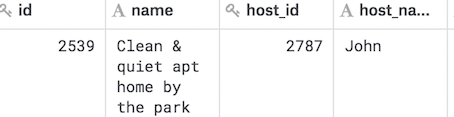
\includegraphics{table_sample.png}

\subsection{Why we choose this dataset}
First of all, this dataset is real-life, every attribute has it's own meaning which make it more practical. 
Secondly, it is not a huge dataset, which means it can be handled more easily yet still challenging. 
Last but not least, it is an open-source dataset having a quite good organization, which is a great instance to explore.

\subsection{What we plan to use this dataset}
\subsubsection{Prediction}
One important usage of data mining is to do predictions, especially for commercial
datasets. For our dataset, the prediction means giving a new Airbnb host with its imformations, 
we should be able to predict its price range with a high probability.
\subsubsection{Evaluation}
Evaluation is also very important in commercial activities. 
There is another attribute called rating which is also a good measure for data mining. 
We can do data mining based on the factors that will influent the rating by doing correlation
analysis. Moreover, some hosts with little numbers of evaluation and high rating should also be taken into consideration. 
\subsubsection{Integration}
We all know that in real life, apart from the data itself, there are many other outside factors that can 
have impact on the data. What we want to do here is to itegrate the data with some other factors
like the map information of the New York City, safety level of the neighborhoods and so on.
In the end, we will try to do visualization of these data to give a more readable and direct result to everyone.

\subsection{How}
Several data mining algorithms that we possibly use are: Decision Tree and Forest, Naive Bayes and Nearest Neighbors.
Programming languages are R and python. But it all depends on futher implementation.

\section{Futher Planning}
Week 9: Preparation and dataset selection(finished)

Week 10-11: Data features anlysis and different algorithms try out

Week 12-13: Run selected algorithm and make improvements on precision and accuracy. Doing visualization and integration.

Week 14: Documentation along with doing presentation. 

\end{document}
